% Options for packages loaded elsewhere
\PassOptionsToPackage{unicode}{hyperref}
\PassOptionsToPackage{hyphens}{url}
%
\documentclass[
]{article}
\usepackage{amsmath,amssymb}
\usepackage{iftex}
\ifPDFTeX
  \usepackage[T1]{fontenc}
  \usepackage[utf8]{inputenc}
  \usepackage{textcomp} % provide euro and other symbols
\else % if luatex or xetex
  \usepackage{unicode-math} % this also loads fontspec
  \defaultfontfeatures{Scale=MatchLowercase}
  \defaultfontfeatures[\rmfamily]{Ligatures=TeX,Scale=1}
\fi
\usepackage{lmodern}
\ifPDFTeX\else
  % xetex/luatex font selection
\fi
% Use upquote if available, for straight quotes in verbatim environments
\IfFileExists{upquote.sty}{\usepackage{upquote}}{}
\IfFileExists{microtype.sty}{% use microtype if available
  \usepackage[]{microtype}
  \UseMicrotypeSet[protrusion]{basicmath} % disable protrusion for tt fonts
}{}
\makeatletter
\@ifundefined{KOMAClassName}{% if non-KOMA class
  \IfFileExists{parskip.sty}{%
    \usepackage{parskip}
  }{% else
    \setlength{\parindent}{0pt}
    \setlength{\parskip}{6pt plus 2pt minus 1pt}}
}{% if KOMA class
  \KOMAoptions{parskip=half}}
\makeatother
\usepackage{xcolor}
\usepackage[margin=1in]{geometry}
\usepackage{color}
\usepackage{fancyvrb}
\newcommand{\VerbBar}{|}
\newcommand{\VERB}{\Verb[commandchars=\\\{\}]}
\DefineVerbatimEnvironment{Highlighting}{Verbatim}{commandchars=\\\{\}}
% Add ',fontsize=\small' for more characters per line
\usepackage{framed}
\definecolor{shadecolor}{RGB}{248,248,248}
\newenvironment{Shaded}{\begin{snugshade}}{\end{snugshade}}
\newcommand{\AlertTok}[1]{\textcolor[rgb]{0.94,0.16,0.16}{#1}}
\newcommand{\AnnotationTok}[1]{\textcolor[rgb]{0.56,0.35,0.01}{\textbf{\textit{#1}}}}
\newcommand{\AttributeTok}[1]{\textcolor[rgb]{0.13,0.29,0.53}{#1}}
\newcommand{\BaseNTok}[1]{\textcolor[rgb]{0.00,0.00,0.81}{#1}}
\newcommand{\BuiltInTok}[1]{#1}
\newcommand{\CharTok}[1]{\textcolor[rgb]{0.31,0.60,0.02}{#1}}
\newcommand{\CommentTok}[1]{\textcolor[rgb]{0.56,0.35,0.01}{\textit{#1}}}
\newcommand{\CommentVarTok}[1]{\textcolor[rgb]{0.56,0.35,0.01}{\textbf{\textit{#1}}}}
\newcommand{\ConstantTok}[1]{\textcolor[rgb]{0.56,0.35,0.01}{#1}}
\newcommand{\ControlFlowTok}[1]{\textcolor[rgb]{0.13,0.29,0.53}{\textbf{#1}}}
\newcommand{\DataTypeTok}[1]{\textcolor[rgb]{0.13,0.29,0.53}{#1}}
\newcommand{\DecValTok}[1]{\textcolor[rgb]{0.00,0.00,0.81}{#1}}
\newcommand{\DocumentationTok}[1]{\textcolor[rgb]{0.56,0.35,0.01}{\textbf{\textit{#1}}}}
\newcommand{\ErrorTok}[1]{\textcolor[rgb]{0.64,0.00,0.00}{\textbf{#1}}}
\newcommand{\ExtensionTok}[1]{#1}
\newcommand{\FloatTok}[1]{\textcolor[rgb]{0.00,0.00,0.81}{#1}}
\newcommand{\FunctionTok}[1]{\textcolor[rgb]{0.13,0.29,0.53}{\textbf{#1}}}
\newcommand{\ImportTok}[1]{#1}
\newcommand{\InformationTok}[1]{\textcolor[rgb]{0.56,0.35,0.01}{\textbf{\textit{#1}}}}
\newcommand{\KeywordTok}[1]{\textcolor[rgb]{0.13,0.29,0.53}{\textbf{#1}}}
\newcommand{\NormalTok}[1]{#1}
\newcommand{\OperatorTok}[1]{\textcolor[rgb]{0.81,0.36,0.00}{\textbf{#1}}}
\newcommand{\OtherTok}[1]{\textcolor[rgb]{0.56,0.35,0.01}{#1}}
\newcommand{\PreprocessorTok}[1]{\textcolor[rgb]{0.56,0.35,0.01}{\textit{#1}}}
\newcommand{\RegionMarkerTok}[1]{#1}
\newcommand{\SpecialCharTok}[1]{\textcolor[rgb]{0.81,0.36,0.00}{\textbf{#1}}}
\newcommand{\SpecialStringTok}[1]{\textcolor[rgb]{0.31,0.60,0.02}{#1}}
\newcommand{\StringTok}[1]{\textcolor[rgb]{0.31,0.60,0.02}{#1}}
\newcommand{\VariableTok}[1]{\textcolor[rgb]{0.00,0.00,0.00}{#1}}
\newcommand{\VerbatimStringTok}[1]{\textcolor[rgb]{0.31,0.60,0.02}{#1}}
\newcommand{\WarningTok}[1]{\textcolor[rgb]{0.56,0.35,0.01}{\textbf{\textit{#1}}}}
\usepackage{graphicx}
\makeatletter
\newsavebox\pandoc@box
\newcommand*\pandocbounded[1]{% scales image to fit in text height/width
  \sbox\pandoc@box{#1}%
  \Gscale@div\@tempa{\textheight}{\dimexpr\ht\pandoc@box+\dp\pandoc@box\relax}%
  \Gscale@div\@tempb{\linewidth}{\wd\pandoc@box}%
  \ifdim\@tempb\p@<\@tempa\p@\let\@tempa\@tempb\fi% select the smaller of both
  \ifdim\@tempa\p@<\p@\scalebox{\@tempa}{\usebox\pandoc@box}%
  \else\usebox{\pandoc@box}%
  \fi%
}
% Set default figure placement to htbp
\def\fps@figure{htbp}
\makeatother
\setlength{\emergencystretch}{3em} % prevent overfull lines
\providecommand{\tightlist}{%
  \setlength{\itemsep}{0pt}\setlength{\parskip}{0pt}}
\setcounter{secnumdepth}{-\maxdimen} % remove section numbering
\usepackage{bookmark}
\IfFileExists{xurl.sty}{\usepackage{xurl}}{} % add URL line breaks if available
\urlstyle{same}
\hypersetup{
  pdftitle={Lab00},
  hidelinks,
  pdfcreator={LaTeX via pandoc}}

\title{Lab00}
\author{}
\date{\vspace{-2.5em}}

\begin{document}
\maketitle

\subsubsection{1. Get acquainted with
RStudio}\label{get-acquainted-with-rstudio}

Read
\href{https://www.gastonsanchez.com/R-ice-breaker/1-07-rstudio-tour.html}{this
short tutorial} (at least the page linked to here, but I recommend
reading other pages in the tutorial as well).

\subsubsection{2. Change global settings in
RStudio}\label{change-global-settings-in-rstudio}

This will prevent some headaches later

\begin{enumerate}
\def\labelenumi{\arabic{enumi}.}
\tightlist
\item
  In the menu bar, go to \texttt{Tools\ \textgreater{}\ Global\ Options}
\item
  Make sure ``Restore .RData into workspace at startup'' is
  \emph{unchecked}
\item
  Set ``Save workspace to .RData'' to ``Never''
\end{enumerate}

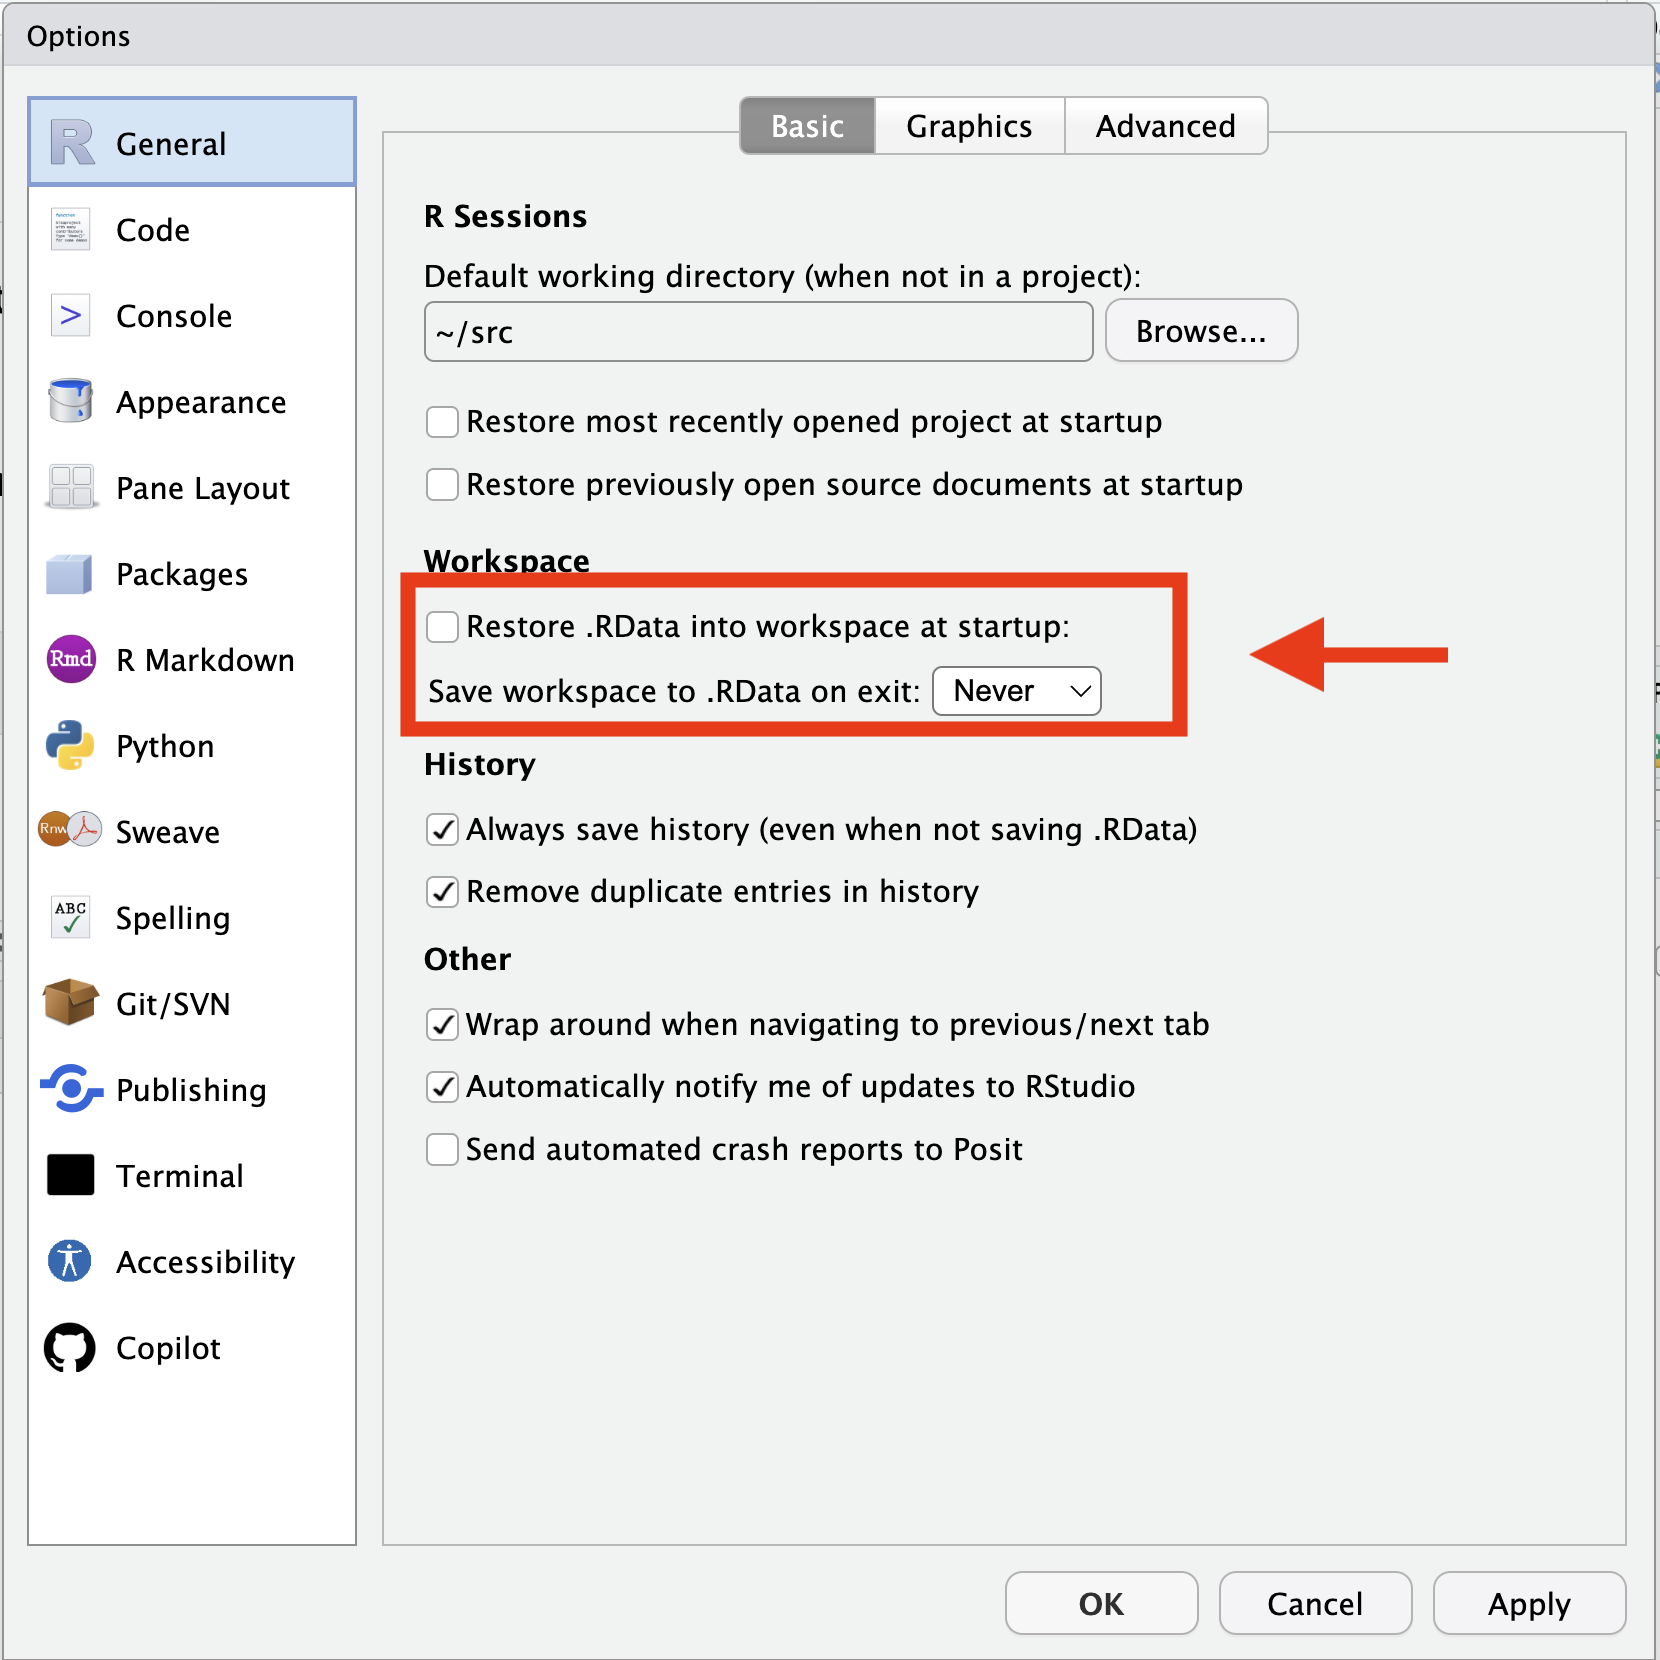
\includegraphics[width=4.16667in,height=\textheight,keepaspectratio]{lab00/r_global_options.png}

\subsubsection{\texorpdfstring{3. Save this file as
\texttt{lab00.Rmd}}{3. Save this file as lab00.Rmd}}\label{save-this-file-as-lab00.rmd}

\texttt{File\ \textgreater{}\ Save}

\subsubsection{4. ``Knit and submit''}\label{knit-and-submit}

When submitting assignments, you do two things

\begin{enumerate}
\def\labelenumi{\arabic{enumi}.}
\tightlist
\item
  You ``knit'' the file to a more presentable format (\texttt{pdf} in
  our case)
\item
  Download the pdf file
\item
  Submit on gradescope
\item
  (You can resubmit as many times as you want, up until the deadline)
\end{enumerate}

\textbf{1. Knitting} \textbf{to pdf}

Just click the ``Knit'' button in the toolbar, which will open a window
with the rendered pdf file

\pandocbounded{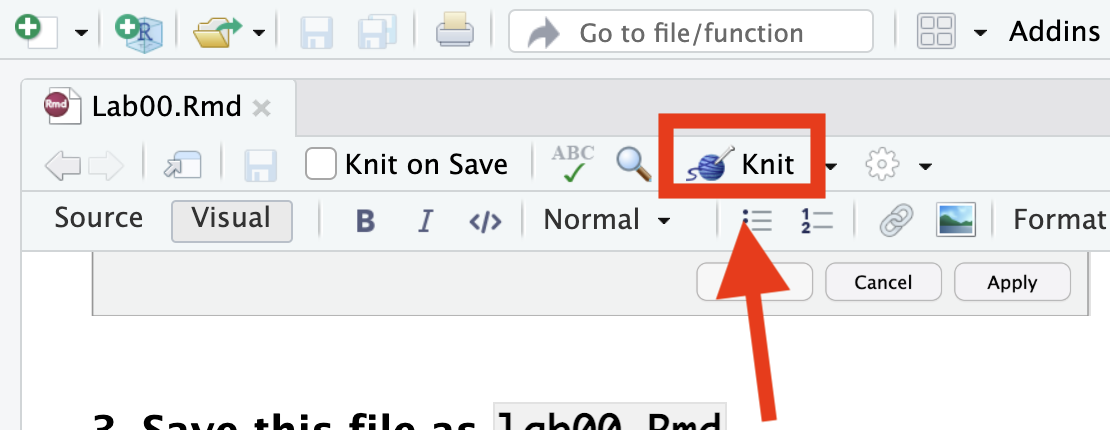
\includegraphics[keepaspectratio]{images/r_knit_button.png}}

You'll see a more ``presentable'' version of the document, like this:

\pandocbounded{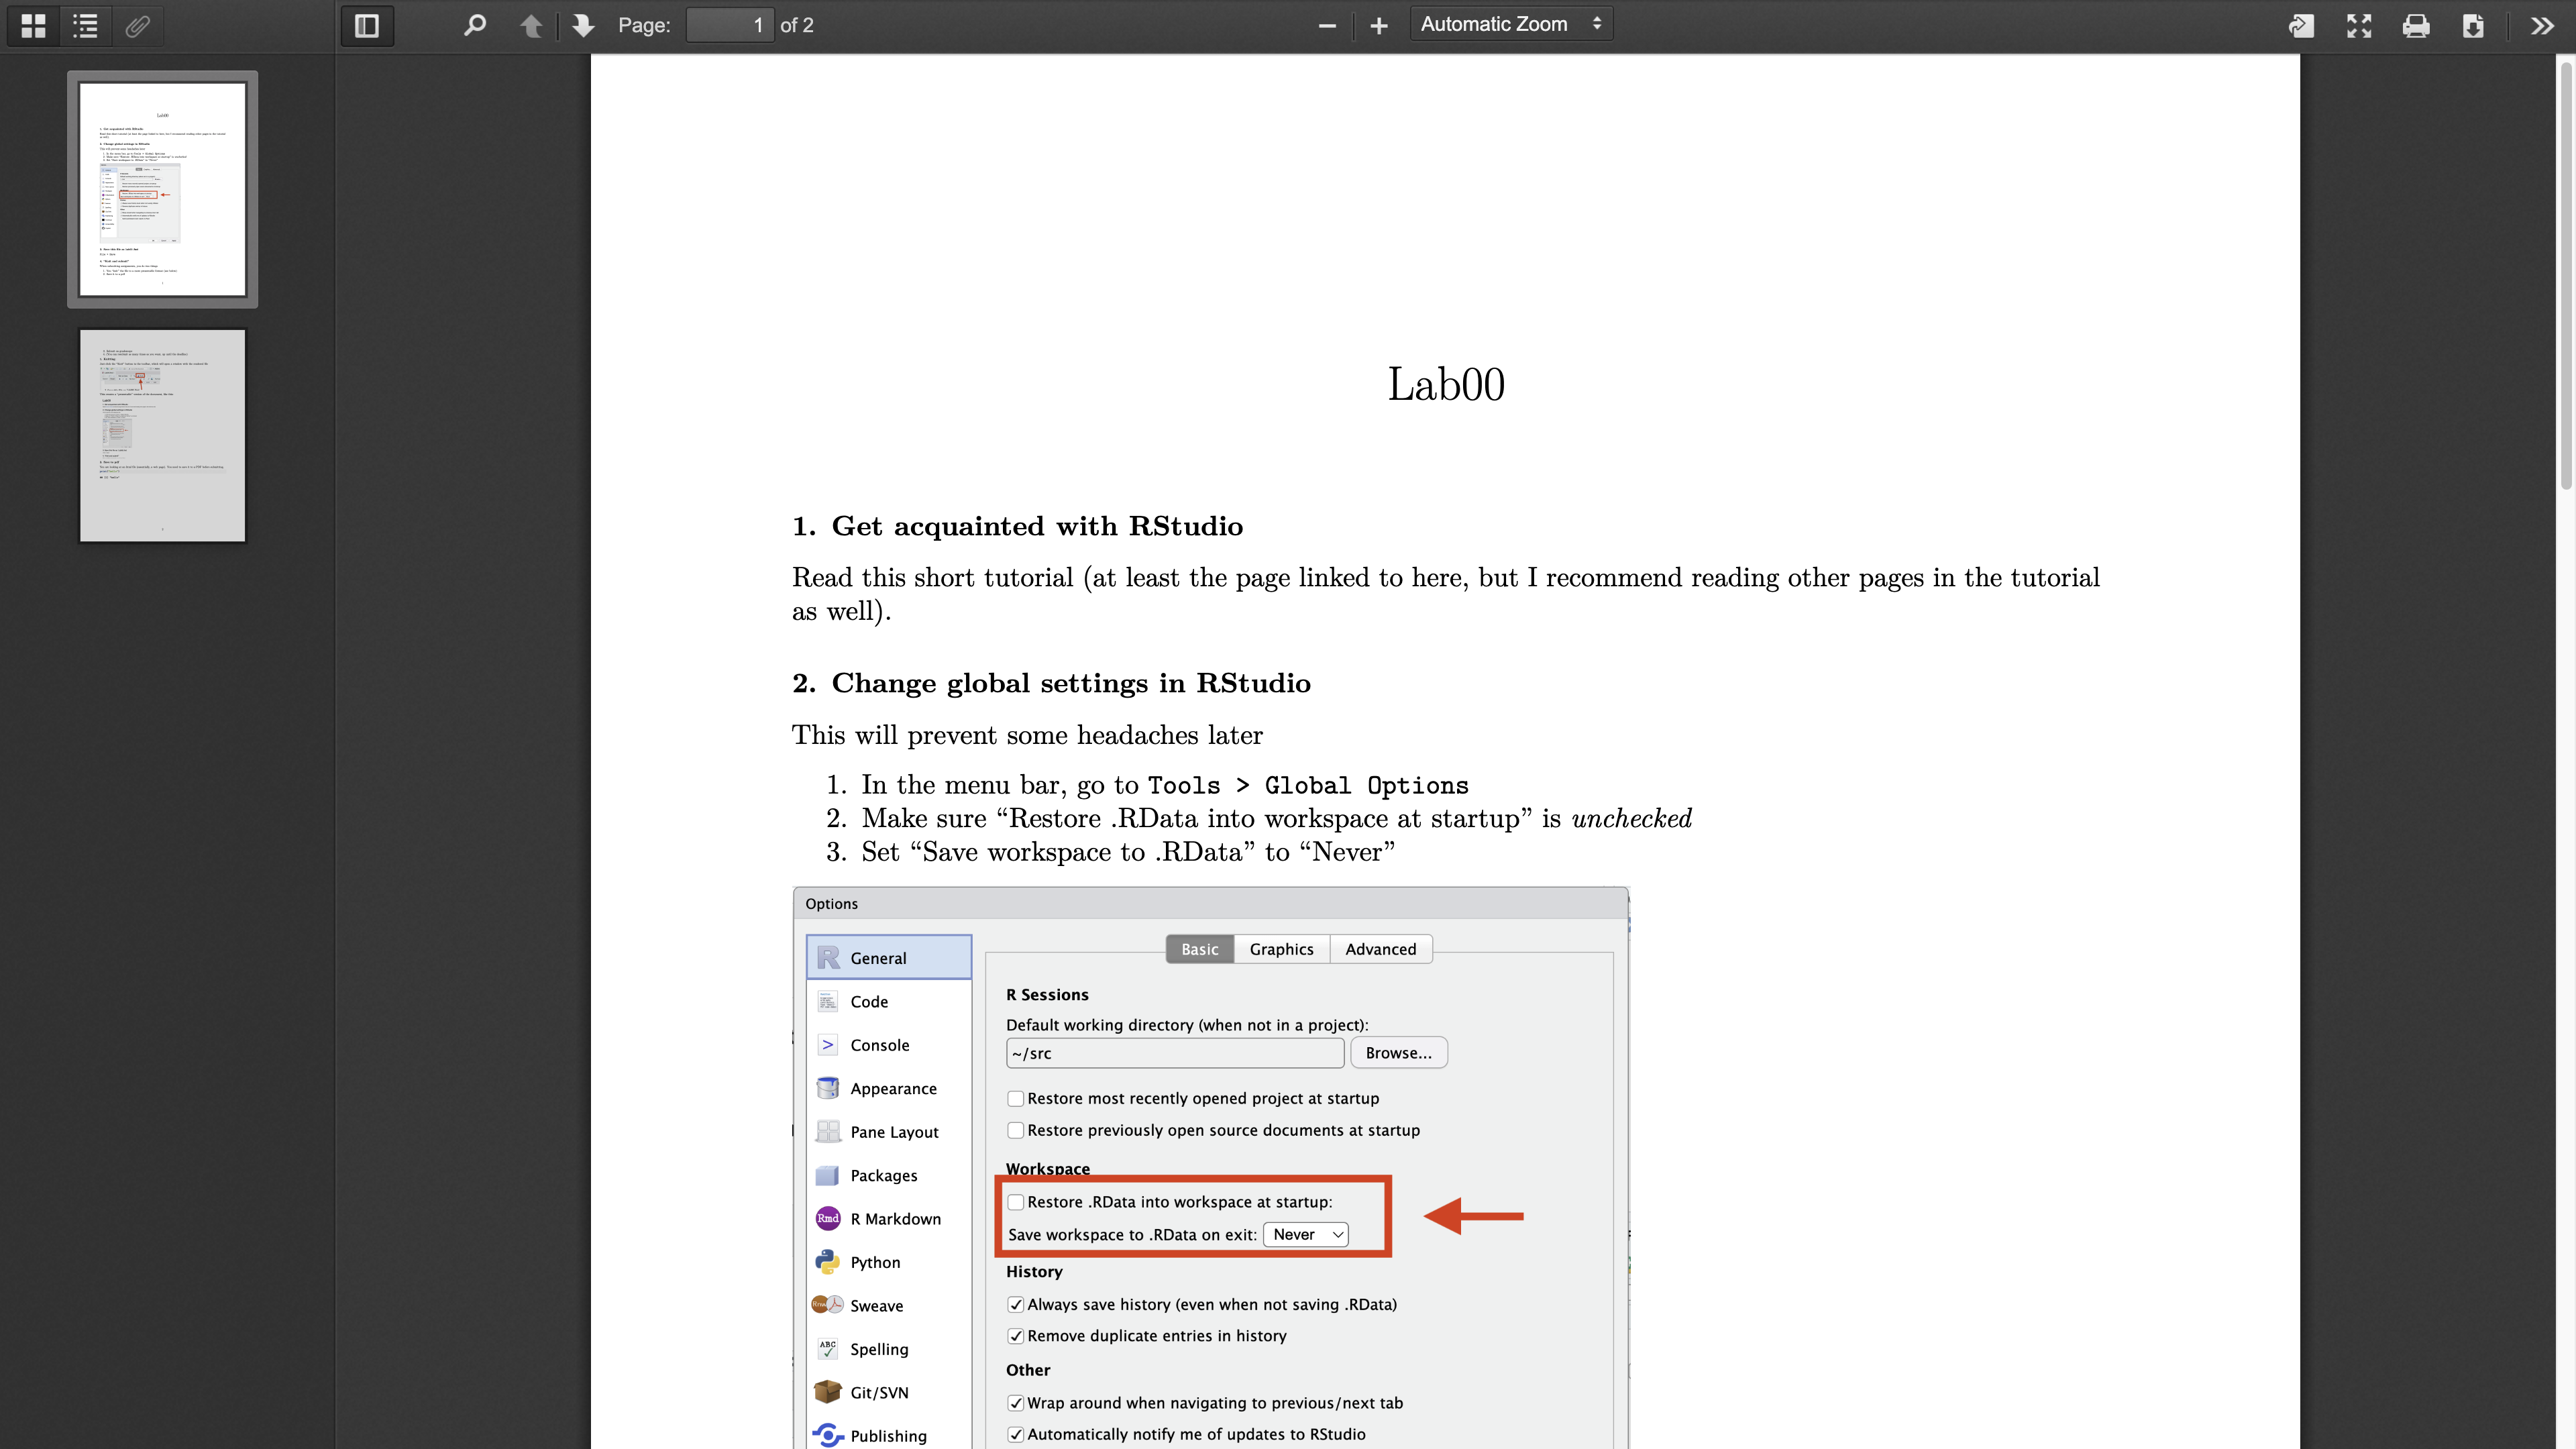
\includegraphics[keepaspectratio]{images/r_rendered_pdf.png}}

\textbf{Notice, in RStudio, you'll now have a \texttt{lab00.pdf}} file:

In the bottom-right \texttt{Files} pane:

\includegraphics[width=2.08333in,height=\textheight,keepaspectratio]{lab00/files_pane.png}

\textbf{2. Download the pdf file}

\textbf{Check the empty checkbox next to the file:}

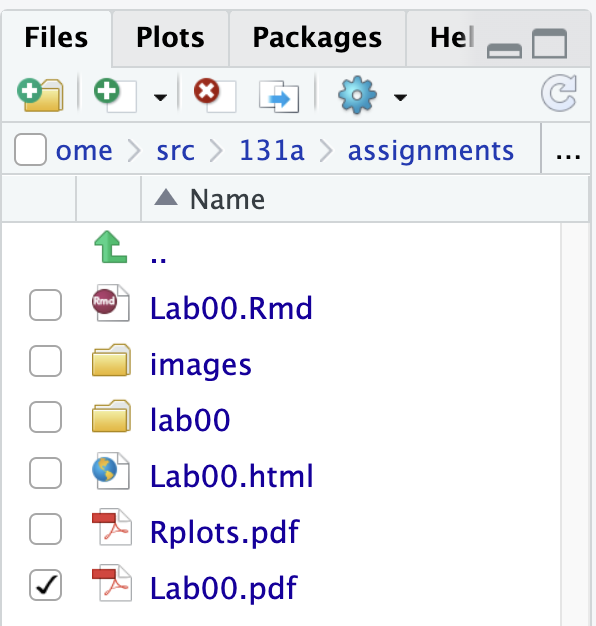
\includegraphics[width=2.08333in,height=\textheight,keepaspectratio]{lab00/files_pane_checkbox.png}

\textbf{Click the Gear (``More'') icon in the \texttt{Files} pane
toolbar and select \texttt{Export}}

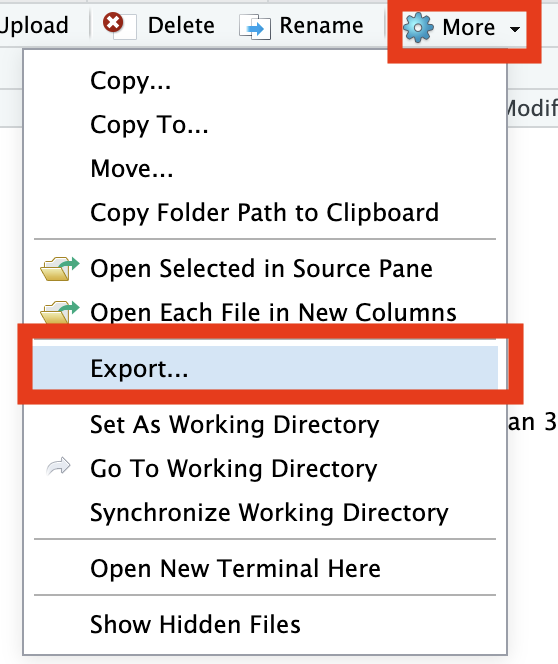
\includegraphics[width=2.08333in,height=\textheight,keepaspectratio]{lab00/files_pane_export.png}

Save somewhere you can find it

\textbf{3. Submit on Gradescope}

\begin{itemize}
\item
  Log into gradescope (go to the course homepage and click
  ``Gradescope'')
\item
  Click on ``assignments''
\item
  Click Lab 00
\item
\end{itemize}

\begin{Shaded}
\begin{Highlighting}[]
\FunctionTok{print}\NormalTok{(}\StringTok{"hello"}\NormalTok{)}
\end{Highlighting}
\end{Shaded}

\begin{verbatim}
## [1] "hello"
\end{verbatim}

\end{document}
